\subsection{Major increase in compartmentalization and disparity after gastrulation}
%objective
With \textit{Ciona}, I measured compartmentalization combining gene expression data at the individual cell-level (until gastrula) or tissue level (tailbud stages) with various 3D embryo models.
Therefore, in here I will refer to relative volume of expression (instead of area as previously)
%results
Globally, the volume of expression decreases mostly after gastrulation (between the 112-cell and the early tailbud stage).
However less dramatic, I found significant differences between the 32-cell and 64-cell stages, and between the 64-cell and 112-cell stages.

As expected, the major increase in disparity happens also occurs between the 112-cell and the early tailbud stage (II, Fig. 4).
I also found a significant increase in disparity in the 64 to 112-cell stages and early to mid-tailbud stages transitions.
Importantly, I found no significant differences between the relative volume of expression of the early and mid-tailbud (II, Fig. 3A), but I found a significant difference between their disparity.

%discussion

This means that, on average, genes are expressed in a similar number of tissues in these stages, but in the mid tailbud the combination of genes expressed in these tissues are more different between each other. This shows that the disparity measure is complementary to the relative volume measure to describe the compartmentalization of the embryo.

In contrast to what I found in \textit{Drosophila}, the major change in compartmentalization in \textit{Ciona} occurs clearly after gastrulation.
In \textit{Ciona}, early embryonic patterning is based on maternal determinants and signalling events mostly between neighbouring cells \citep{Lemaire2009}, which act in a combinatorial way \citep{Hudson2007} to establish a unique TF combination in more than half of the blastomere pairs before gastrulation \citep{Imai2006} determining most of their fates.
Thus, even when in \textit{Ciona} most of the cell fates are already determined (by the specific combination of a fraction of TFs) and the embryo can be said to be already highly compartmentalized, this is not evident at the global level of gene expression, which I am measuring here.
This `delay' could be explained by the relatively slower process of signal transduction (as in \textit{Ciona}) compared to the gap gene network (in \textit{Drosophila}).

%%%%%%%%%%%%%%%%%%%%%%%%%%%%%%%%%%%%%%%%%%%%%%%%%%%%%%%%%%%%%%%%%%%%%%%%%%%%%%%%%%%%% 
\subsection{The leading role of TFs and SIGs}
%objective
I then tested if in \textit{Ciona} the TFs and signalling molecules (SIGs) also showed an early compartmentalization, expected from their allegedly leading role in early pattern formation.
	\nomenclature{SIGs}{Signaling molecules}
	\nomenclature{RTK}{receptor tyrosine kinase}
SIGs consist of genes of receptor tyrosine kinase (RTK) pathways such as FGFs and intracellular signalling molecules such as MAPK, Notch, Wnt, TGF$\beta$, Hedgehog and genes in the JAK/STAT pathways (based on \citealp{Imai2004}) 

%results 1
As expected, TFs volume of expression decreased faster than non-TFs. The TFs showed lower volume of expression in the 64-cell and 112-cell stages (II, Fig. 3B). The results are similar for maternal and zygotic genes (maternal/zygotic classification based on \citealp{Matsuoka2013}; II,Fig. S1).
I then compared TF families (categories based on \citealp{Imai2004}) and found that six TF families showed lower relative volume in the early gastrula (BZIP, T-box, bHLH, HMG, Nuclear Receptor, and `Other-TFs') but only T-box genes showed a lower relative volume from the 32-cell stage until gastrula (II,Fig. S2). 

%discussion 1
The results obtained for the T-box gene family (conserved in metazoan and several non-metazoan lineages \citep{Sebe-Pedros2013}) are consistent with the known important role these genes have in diverse metazoan species early cell fate specification (reviewed in: \citealp{Papaioannou2014,Showell2004}.
Examples of T-box genes in \textit{Ciona} are Tbx6 and \textit{brachyury}, crucial for muscle tissue formation \citep{Mitani1999,Nishida2005} and for notochord specification \citep{Yasuo1998}, respectively.
 
%results 2
SIGs showed significant lower relative volume of expression than the rest of the genes in the 32-cell, 64-cell, and 112-cell stages (II, Fig. 3B).
Specifically, in the 64-cell stage RTK-MAPK, Wnt and TGF$\beta$ families showed significant higher disparity in the 64 cells stage, suggesting a predominant role of these pathways in the patterning of the embryo at this stage. 
%discussion2
This is consistent with known short range induction events by nodal and various FGFs, which are part of the TGF$\beta$ and RTK-MAPK signalling pathways, respectively \citep{Lemaire2008}.
%general discussion? (X)


%%%%%%%%%%%%%%%%%%%%%%%%%%%%%%%%%%%%%%%%%%%%%%%%%%%%%%%%%%%%%%%%%%%%%%%%%%%%%%%%%%%%% 
\subsection{3D roughness increases non-linearly}
%objective
In here I used the Dirichlet Normal Energy (DNE; \citealp{Winchester2016}) as a measure of complexity that considers the overall curvature of the 3D surface of a gene expression pattern.
Importantly, DNE can also be analysed at different spatial scales. 
	\nomenclature{DNE}{Dirichlet Normal Energy}
Therefore, DNE would be the 3D equivalent of the roughness measure I used for \textit{Drosophila}.

%results
DNE values increase throughout development (II, Fig. 5), again with the major change between the 112-cell and the early tailbud. 

The max (mean of the last decile) values increase substantially already between the 64 and 112 cells stages (with 1000 and 10000 polygonal faces), while the min values (mean of the first decile) remain practically constant during development, showing that the most complex patterns in each stage get increase their DNE value but there is always a proportion of very simple expression pattern.
Also, I found that at low spatial scales (1000 and 10000 polygons per mesh; II, Fig. 5) I found that the mean DNE of the late tailbud is higher than at the mid tailbud (one-way ANOVA pvals < 0.05).
	\nomenclature{ANOVA}{Analysis of Variance}

%discussion
In summary, this results show that the complexity of distribution in 3D space of cells/tissues expressing a gene (measured with DNE) increases through development, as even when the increase was more pronounced just after gastrulation, significant changes were found before and after this.

%%%%%%%%%%%%%%%%%%%%%%%%%%%%%%%%%%%%%%%%%%%%%%%%%%%%%%%%%%%%%%%%%%%%%%%%%%%%%%%%%%%%% 
\subsection{Synexpression territories in \textit{Ciona}}
%objective
Because in the tailbud stages the information is based on tissues and not on individual cells as the early stages, I analysed the synexpression territories (STs) of these stages separately by means of a hierarchical clustering (II, Methods). As in Drosophila, how the different STs cluster with each other is informative of the degree of differentiation between stages. If STs cluster with other STs in the same stage, it would mean that the majority of genes change their expression in a similar way over time independently of where they are. If STs cluster with other STs in the same part of the
embryo in successive stages, it would mean that this part of the embryo has expression dynamics independent from other parts of the embryo, which would be expected in already differentiated cells/tissues.

%results
Early stages STs cluster by stage. Thus, even if at the first three stages a high proportion of blastomeres express a nearly unique combination of transcriptional factors \citep{Imai2006}, the bulk change in gene expression is common to all blastomeres. Within each early stage, STs coincides very well with the know fate map (II, Fig 6A; II, Fig. S8), with some exceptions That I describe in the next subsection.

In contrast, in tailbud stages practically all STs cluster by tissue/cell type, which indicates that the in early tailbud, most tissues are already quite differentiated.
This is largely consistent with the bulk of other studies analyzing these stages at the level of individual or small sets of genes \citep{Corbo1997,DiGregorio1999}.

%discussion 2
The early stages analysis is similar to one made by \citet{Imai2006}, who used the expression profile of 53 zygotically TFs in single cells in the 16, 32, 64, and 112-cell stages, to perform a hierarchical clustering (for each stage separately). My analysis is different in two aspects: I performed the clustering using the blastomeres of different stages and my analysis is not restricted to TFs. As I said previously, using various stages is informative of the overall differentiation process and can be used to discern between differentiation scenarios, as the differences between early and tailbud stages I found here.

\begin{figure}[h]
  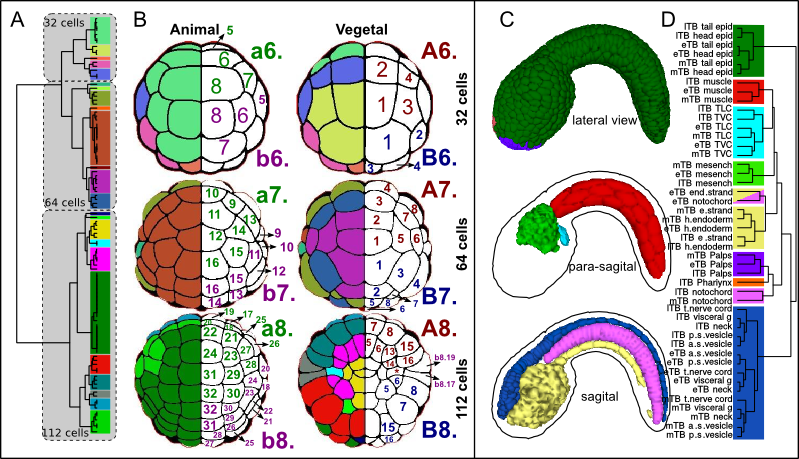
\includegraphics[width=\textwidth]{./Images/Art-II/territories.png}
  \centering
  \caption{Ciona synexpression territories. 
  (A) Dendrogram produced by hierarchical clustering of cells in 32-cell, 64-cell and 112-cell stages. Dashed boxes show that STs cluster by stage. Coloured boxes show the cut-off to produce 24 STs.
  (B) Names of cells (Conklin nomenclature; \citealp{Conklin1905}) indicated with a prefix shown at right. STs in the 32 cells, 64 cells and 112 cells stages (top, middle and bottom, respectively). Colour refers to which ST of the dendrogram (in A) each cell is part of. Animal view based on \citet{Nicol1988} and vegetal view based on \citet{Cole2004a}. The cell marked with a star (*) is the A7.6 cell, that in this analysis represents their descendant cells (A8.11 and A8.12).
  C) Dendrogram produced by hierarchical clustering of tissues in early, mid and late tailbud stages. The coloured boxes show the cutoff to produce 10 STs. (D) STs in the tailbud stages shown in a lateral, para-sagital and sagital views of a mid tailbud 3D embryo model (from \citealp{Nakamura2012}). Colour refers to which ST of the dendrogram (in C) each tissue is part of.
}
  \label{fig:Art-II-territories}
\end{figure}

%%%%%%%%%%%%%%%%%%%%%%%%%%%%%%%%%%%%%%%%%%%%%%%%%%%%%%%%%%%%%%%%%%%%%%%%%%%%%%%%%%%%% 
\subsection{Discrepancies between fate map and STs}

I found a few cases in which cells with the same fate where contained in different STs. This would be the case of: 1) cells whose fate is disproportionally affected or determined by a small number of genes (as this analysis reflect quantitative differences at the level of hundreds of expressed genes
but can not distinguish between the relative importance of each gene) or 2) cells that although having a restricted fate at a certain stage their differentiation is not complete (at the level of gene expression).

An example of the latter is a ST in the 112-cell stage (in magenta; Fig. X) that contains   precursors of the notochord (A8.5, A8.6, A8.13, and A8.14, B8.6) and mesenchyme (B8.5) \citep{Tokuoka2004}.
The latter come from a secondary notochord/mesenchyme bipotential cell (B7.3). It has been reported that the expression of Twist-like 1, necessary for mesenchyme differentiation, starts at this stage \citep{Imai2003}.
This evidence, together with the inclusion of the mesenchyme cell in this otherwise exclusively notochord territory (primary and secondary), seems to indicate that the differentiation of cell pair B8.5 as mesenchyme is still incomplete at this stage.

\subsection{Gene expression dynamics in cell-lineages}

I analysed the gene expression similarity between lineage-related cells (i.e., between daughters cells and between mother/descendants cells) in the early stages (II, Fig. 8).
In general, cells are more closely genetically to their sister cells than to their mother/descendants, which is reflected in the clustering of STs by stages discussed before.
I found also that at the 64-cell stage, cells that show more genes expressed differently than
their ancestors are neural fated cells, which might be related with the fact the unrestricted state of these cells at this stage (i.e., their descendants will give rise to different cell fates).